\documentclass[12pt, a4paper]{article}
\setlength{\textheight}{24cm}
\setlength{\textwidth}{16cm}
\setlength{\topmargin}{0cm}
\setlength{\evensidemargin}{0cm}
\setlength{\oddsidemargin}{0cm}
\usepackage[affil-it]{authblk}
\usepackage{graphics}
\usepackage{graphicx}
\usepackage{caption}
\usepackage{float}
\usepackage[british]{babel}
\usepackage{hyperref}
\usepackage{subcaption}
\date{}
\begin{document}
\title{Comparison of several frameworks for general-purpose programming and the  computation of FFTs on GPUs}
\author{Philippe Gambron \thanks{\texttt{philippe.gambron{@}stfc.ac.uk}}, Sue Thorne \thanks{\texttt{sue.thorne{@}stfc.ac.uk}}}
\affil{Science and Technology Facilities Council, Hartree Centre, Rutherford Appleton Laboratory, Harwell Campus, Harwell Oxford, OX11 0QZ, United Kingdom}
\maketitle
\begin{abstract}
We compare the performance of several frameworks that can be used, in C, for general-purpose programming on a graphical processing unit (GPU) or to compute Fast Fourier Transforms (FFTs).  
\end{abstract}
\section{Introduction}
For a bit more than a decade, the use of GPU has become increasingly widespread. They are indeed capable of significantly increasing the performance of a single workstation or compute node. While there are some overheads associated to the data transfers between the memory and the GPU and the launch of the kernel and some constraints on the types of algorithms can be efficiently programmed, one can obtain tremendous performance gains on suitable problems.\\

In this report, we will compare the performance of several of these frameworks that we measured for a simple general-purpose programming example and for computing FFTs on the GPU by using the libraries provided by these frameworks. 

\section{Overview of the chosen libraries}
We consider the following frameworks for GPU programming: CUDA \cite{cuda}, OpenCL \cite{opencl}, OpenMP \cite{openmp}\footnote{From version 4.0, OpenMP offers GPU programming} and Kokkos \cite{kokkos}. The first three of these frameworks provide as well FFT libraries. Respectively, they are: cuFFT \cite{cufft}, clFFT \cite{clfft} and AccFFT \cite{accfft} (Table \ref{ffttable}). They can perform complex transforms, real-to-half-complex ones (and conversely) as well as, in the case of FFTW, real-to-real transforms when the signal is odd or even. The half-complex output consists in half as many complex values as there were points in the signal, taking advantage of the hermiticity of the Fourier transform of a real function.\\ 
\begin{table}[H]
\captionsetup{width=1\textwidth}
\begin{tabular}{|p{2.5cm}||p{2.5cm}|p{1cm}|p{3cm}|p{3cm}|p{2cm}|p{2cm}|}
\hline
& Type & Dim. & Radices & Licence \\
\hline
\hline
AccFFT & R$\to$H,\ \ \  C$\to$C& 3& & GPL v2\\
\hline
clFFT  &  R$\to$H,\ \ \  C$\to$C,\ \ \ \  H$\to$R& 1, 2, 3 & 2, 3, 5, 7 & Proprietary\\
\hline
cuFFT  &  R$\to$H,\ \ \  C$\to$C,\ \ \ \  H$\to$R & 1, 2, 3 & 2, 3, 5, 7 & GPL v3\\
\hline
\end{tabular}
\caption{Overview of the FFT libraries considered. R stands for real, C, for complex, and HC, for half-complex.}
\label{ffttable}
\end{table}
\section{Benchmark}
The benchmark \cite{code} consists in calculating the FFT of a series of volumes, in 1, 2 or 3 dimensions, of real or complex values. The purpose was to mimick a problem submitted to us by the CCP PET-MR collaboration \cite{ccppetmr}, within the Software Outlook initiative \cite{softwareoutlook}, who needed to take the transform of series of square complex images. This example is depicted in Fig. \ref{benchmark}. For our more general test, the 2-dimensional slices could be replaced by a line or a rectangular cuboid. We used 32 images, which was a typical value used by that collaboration, for the tests that were representative of their requirement. For the other runs, we always processed a single image.\\

\begin{figure}[H]
\captionsetup{width=0.6\textwidth}
\centering
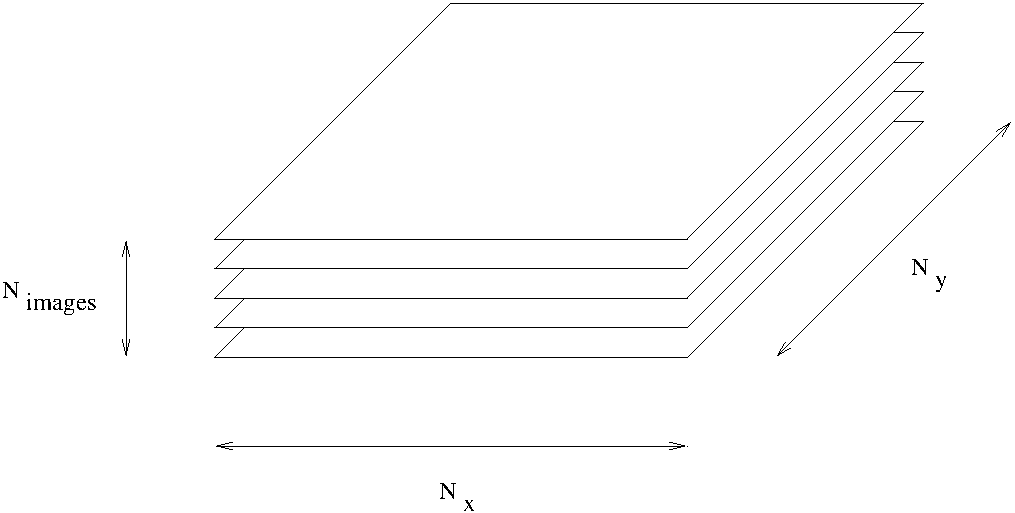
\includegraphics[height=5cm]{benchmark.pdf}
\caption{The benchmark consists in taking the FFT of several images. Each of them is made of real or complex values and can be a simple line, a rectangle or a cuboid.}
\label{benchmark}
\end{figure}

We used a number of points varying from $\sim 10^3$ to $\sim 10^7$. The domains had sides of equal lengths (square or cubic) or were flattened (rectangle or cuboid). These dimensions could be powers of 2, products of powers of small integers (2, 3, 5 and 7) or prime numbers. The values appearing in the graphs are the execution times averaged over 10 runs. The bumps remaining on the graphs in some cases appear consistently when we repeat the measurements.

\section{Setup}

The measurements were carried out on a system featuring an Intel Xeon W-2133 CPU (6 cores, 3.6 GHz), a NVIDIA Quadro GV100 GPU and 12 GB of RAM. We used the following frameworks: CUDA (version 10.0.130), OpenCL (version 1.2.7), OpenACC (version 2.7), OpenMP (version 4.0.0) and Kokkos (version 2.9.0) and clFFT (version 2.0).  

\section{Product}
We first compare the multiplication of an array of $2^{24}$ real or complex numbers by an array of real numbers by considering the operation executed respecively in a serial way on the processor, in a multi-threaded way on the processor as well using OpenMP and Kokkos, on the GPU using CUDA, OpenCL, OpenACC, OpenMP and Kokkos. In the case of CUDA and OpenCL, we have made the comparison using streams or queues. This is a mechanism that allows the concurrent execution of kernels as well as overlapping data transfers in different directions. We observe that the best performance is obtanined with OpenMP, both on the CPU and the GPU.\\

We noted that the example involving with Kokkos was relatively complicated to compile. An external makefile as well as a header file containing the configuration must be included. This will produce, during compilation, sevral object files in the current directory that will have to be linked to produce our executable file. 
\begin{figure}[H]
\captionsetup{width=0.8\linewidth}
\centering
\begin{subfigure}{.5\textwidth}
\centering
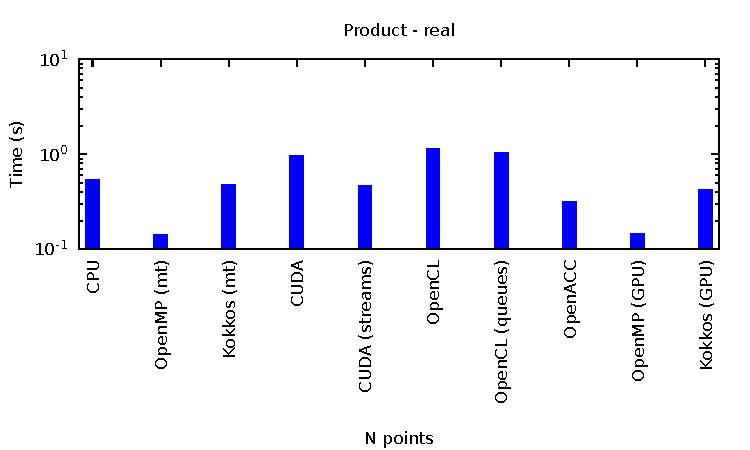
\includegraphics[width=.9\linewidth]{graphs/product-r.pdf}
\caption{Real numbers}
\label{PRODR}
\end{subfigure}%
\begin{subfigure}{.5\textwidth}
\centering
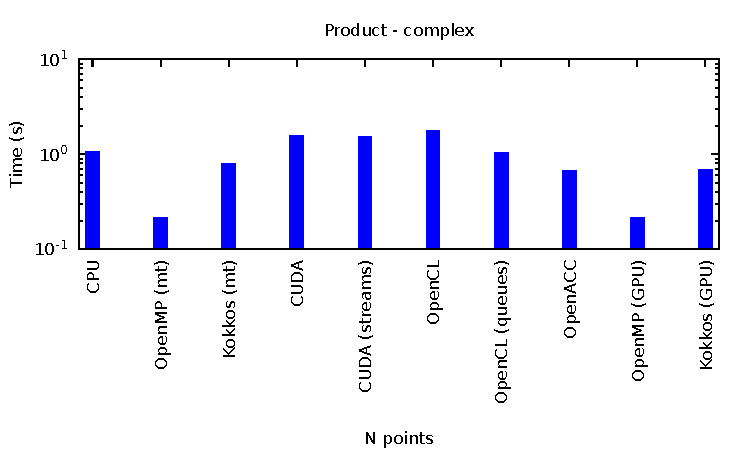
\includegraphics[width=.9\linewidth]{graphs/product-c.pdf}
\caption{Complex numbers}
\label{PRODC}
\end{subfigure}
\caption{Execution time for the product of a large number of $2^{24}$ real and complex points using several frameworks.}
\label{1DFFTW}
\end{figure}



\section{Fast Fourier Transform}
We measure the initialisation and execution times obtained in computing the FFT transform with CUDA, OpenCL and OpenACC for signals that were real and complex in one, two and three dimensions. We consider domains whose sides are identical\footnote{We will study the effect of flattening the domain in .} and that contain a number of points varying from $\sim 10^3$ to $\sim 10^7$. More precisely, we consider numbers of points, on each side, that are a power of two, a product of small integers (2, 3, 5 and 7) and a prime number. \\

As expected, in most cases, we obtain a better performance with a number of points that is a power of 2 or the product of small integers than with primes. CUDA and OpenCL also tend to be more efficient than OpenACC. On the other had, OpenCL suffers from another drawback. While, with the two other frameworks, the initialisation time increases as a function of the domain size, it remains constant and quite large with OpenCL. It can be close and, in some cases, even larger than the execution time.
  
\begin{figure}[H]
\captionsetup{width=0.8\linewidth}
\centering
\begin{subfigure}{.5\textwidth}
\centering
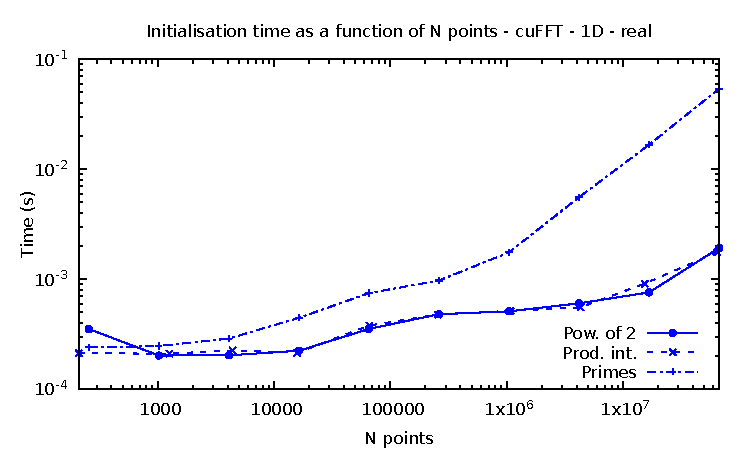
\includegraphics[width=.9\linewidth]{graphs/fft-cuda-1d-pow2-r-init.pdf}
\caption{Intialisation (real)}
\label{FFTCUDA1DRI}
\end{subfigure}%
\begin{subfigure}{.5\textwidth}
\centering
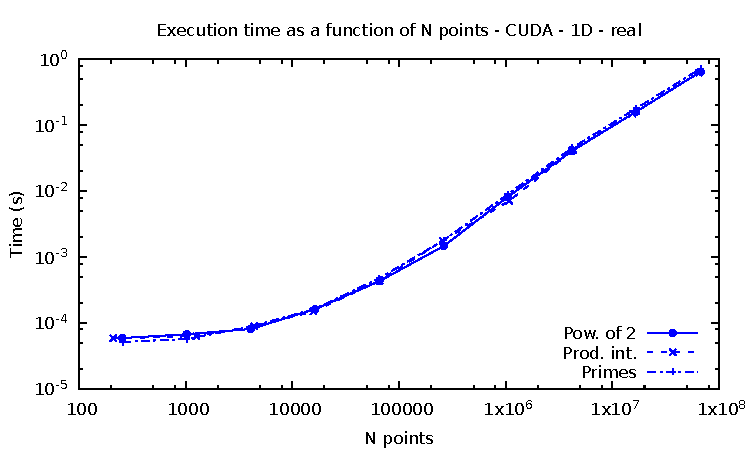
\includegraphics[width=.9\linewidth]{graphs/fft-cuda-1d-pow2-r-exec.pdf}
\caption{Execution (real)}
\label{FFTCUDA1DRE}
\end{subfigure}\\
\begin{subfigure}{.5\textwidth}
\centering
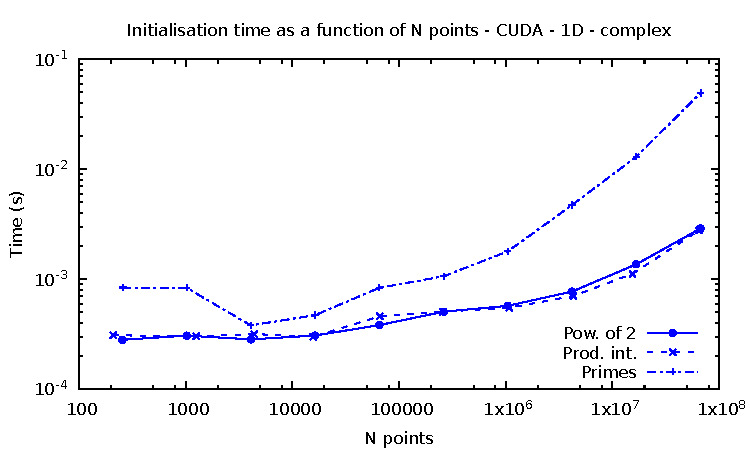
\includegraphics[width=.9\linewidth]{graphs/fft-cuda-1d-pow2-c-init.pdf}
\caption{Intialisation (complex)}
\label{FFTCUDA1DCI}
\end{subfigure}%
\begin{subfigure}{.5\textwidth}
\centering
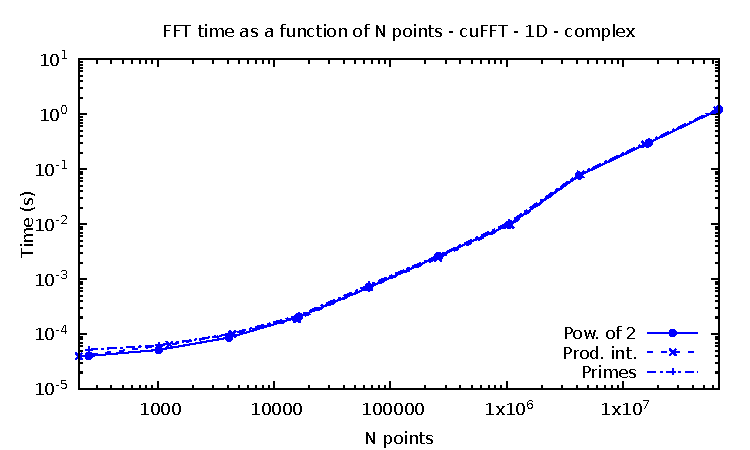
\includegraphics[width=.9\linewidth]{graphs/fft-cuda-1d-pow2-c-exec.pdf}
\caption{Execution (complex)}
\label{FFTCUDA1DCE}
\end{subfigure}
\caption{Initialisation and execution times as a function of the number of points (CUDA, 1 dimension)}
\label{FFTCUDA1D}
\end{figure}


\begin{figure}[H]
\captionsetup{width=0.8\linewidth}
\centering
\begin{subfigure}{.5\textwidth}
\centering
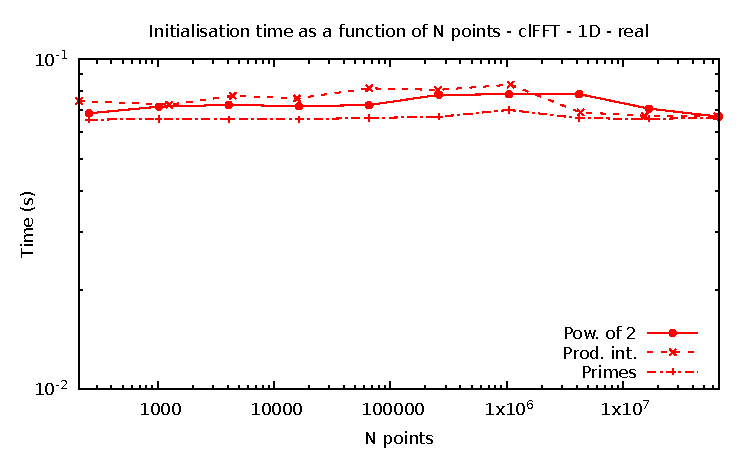
\includegraphics[width=.9\linewidth]{graphs/fft-opencl-1d-pow2-r-init.pdf}
\caption{Intialisation (real)}
\label{FFTCL1DRI}
\end{subfigure}%
\begin{subfigure}{.5\textwidth}
\centering
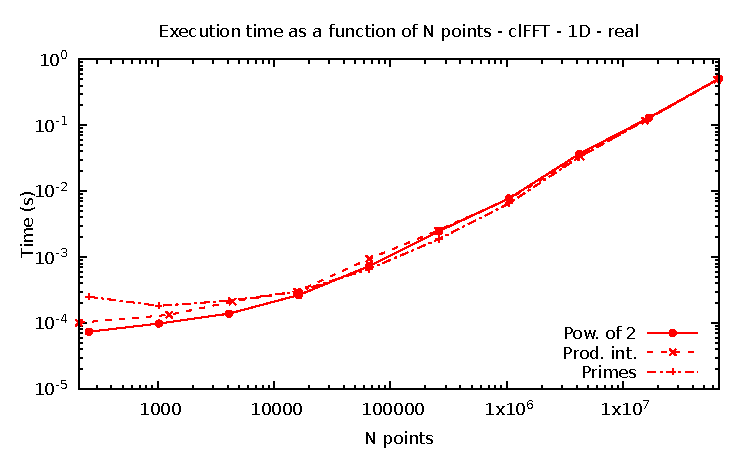
\includegraphics[width=.9\linewidth]{graphs/fft-opencl-1d-pow2-r-exec.pdf}
\caption{Execution (real)}
\label{FFTCL1DRE}
\end{subfigure}\\
\begin{subfigure}{.5\textwidth}
\centering
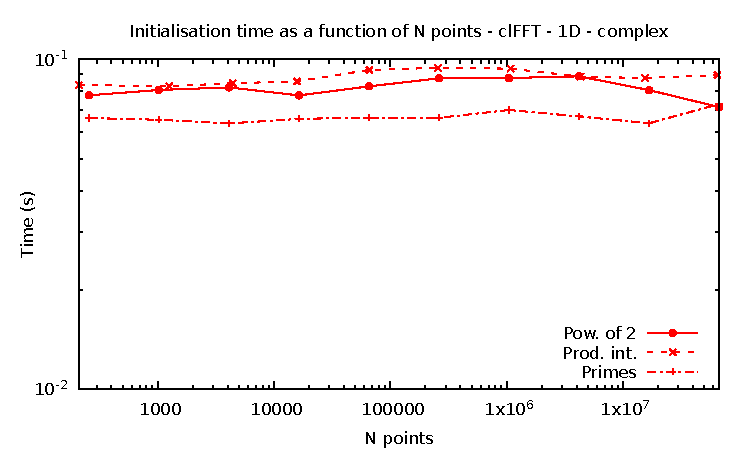
\includegraphics[width=.9\linewidth]{graphs/fft-opencl-1d-pow2-c-init.pdf}
\caption{Intialisation (complex)}
\label{FFTCL1DCI}
\end{subfigure}%
\begin{subfigure}{.5\textwidth}
\centering
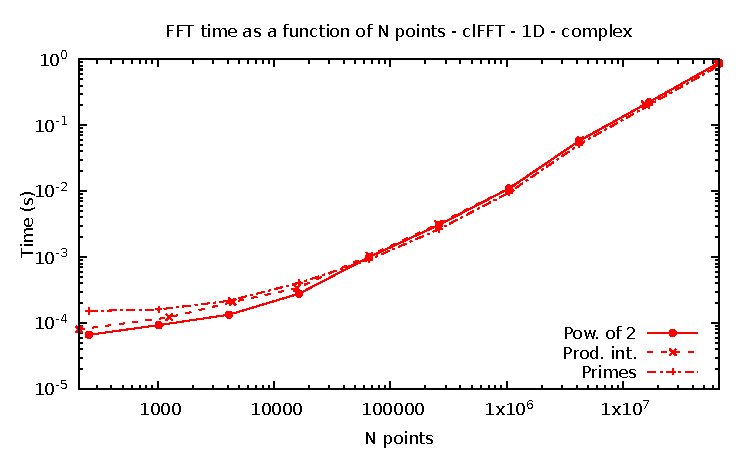
\includegraphics[width=.9\linewidth]{graphs/fft-opencl-1d-pow2-c-exec.pdf}
\caption{Execution (complex)}
\label{FFTCL1DCE}
\end{subfigure}
\caption{Initialisation and execution times as a function of the number of points (OpenCL, 1 dimension)}
\label{FFTCL1D}
\end{figure}

\begin{figure}[H]
\captionsetup{width=0.8\linewidth}
\centering
\begin{subfigure}{.5\textwidth}
\centering
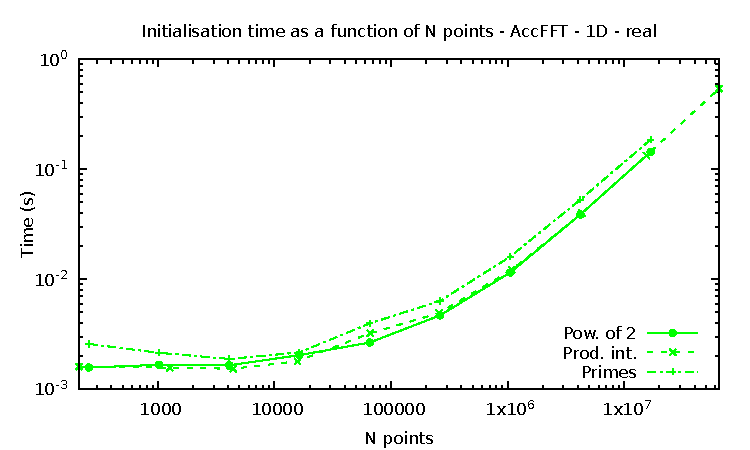
\includegraphics[width=.9\linewidth]{graphs/fft-openacc-1d-pow2-r-init.pdf}
\caption{Intialisation (real)}
\label{FFTACC1DRI}
\end{subfigure}%
\begin{subfigure}{.5\textwidth}
\centering
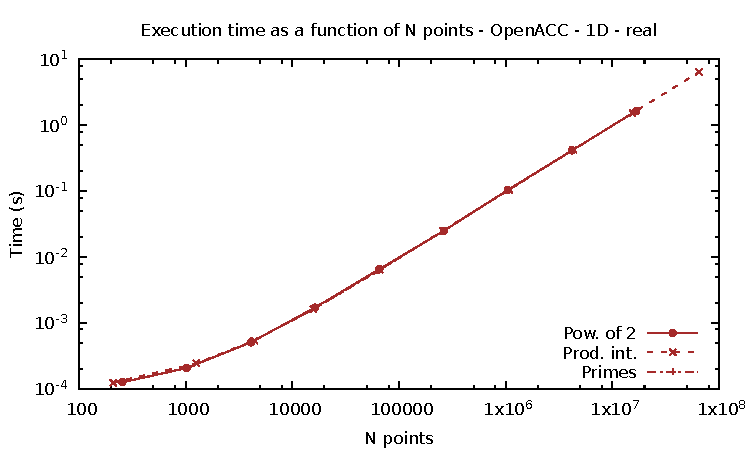
\includegraphics[width=.9\linewidth]{graphs/fft-openacc-1d-pow2-r-exec.pdf}
\caption{Execution (real)}
\label{FFTACC1DRE}
\end{subfigure}\\
\begin{subfigure}{.5\textwidth}
\centering
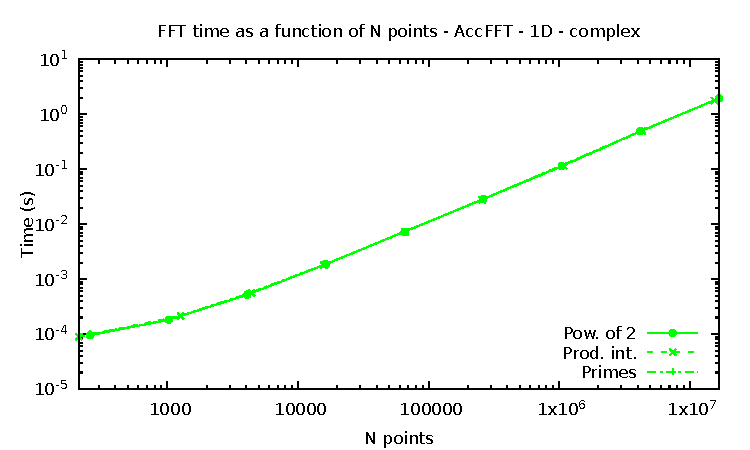
\includegraphics[width=.9\linewidth]{graphs/fft-openacc-1d-pow2-c-exec.pdf}
\caption{Intialisation (complex)}
\label{FFTACC1DCI}
\end{subfigure}%
\begin{subfigure}{.5\textwidth}
\centering
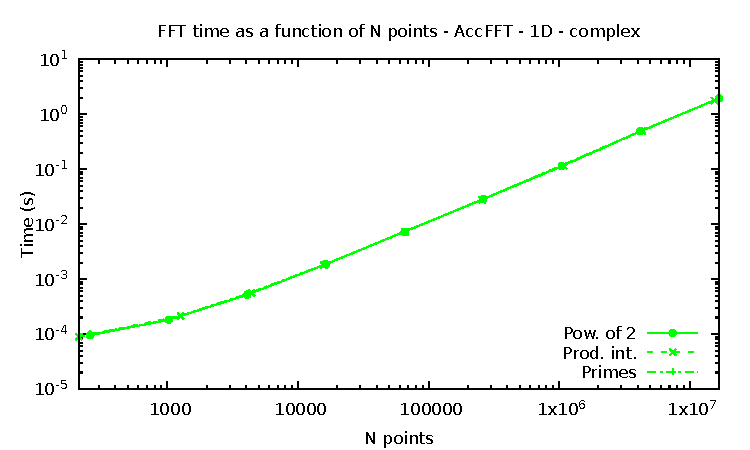
\includegraphics[width=.9\linewidth]{graphs/fft-openacc-1d-pow2-c-exec.pdf}
\caption{Execution (complex)}
\label{FFTACC1DCE}
\end{subfigure}
\caption{Initialisation and execution times as a function of the number of points (OpenACC, 1 dimension)}
\label{FFTCL1D}
\end{figure}


\begin{figure}[H]
\captionsetup{width=0.8\linewidth}
\centering
\begin{subfigure}{.5\textwidth}
\centering
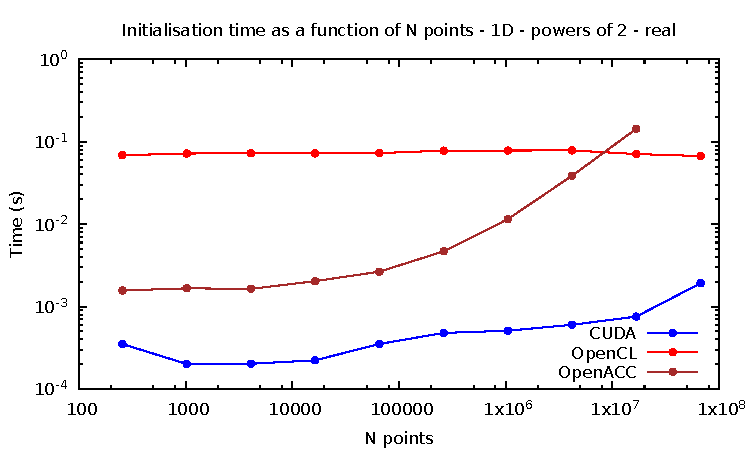
\includegraphics[width=.9\linewidth]{graphs/fft-1d-pow2-r-init.pdf}
\caption{Intialisation (real)}
\label{FFTPOW21DRI}
\end{subfigure}%
\begin{subfigure}{.5\textwidth}
\centering
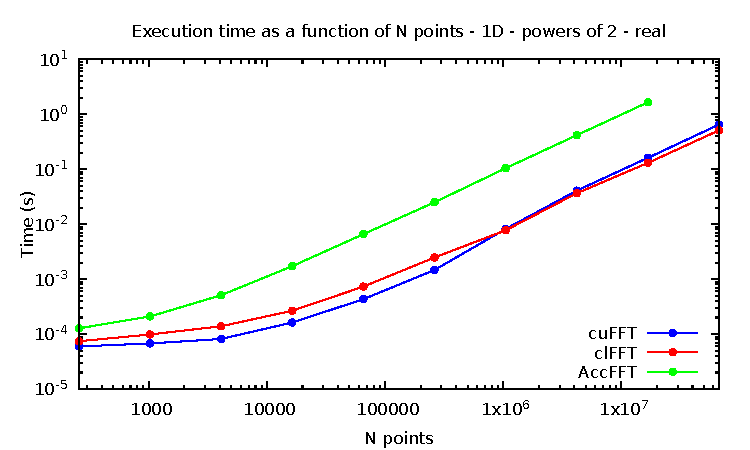
\includegraphics[width=.9\linewidth]{graphs/fft-1d-pow2-r-exec.pdf}
\caption{Execution (real)}
\label{FFTPOW21DRE}
\end{subfigure}\\
\begin{subfigure}{.5\textwidth}
\centering
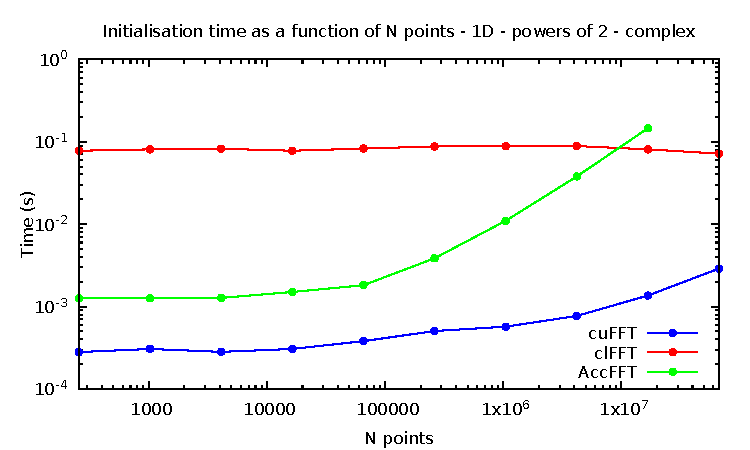
\includegraphics[width=.9\linewidth]{graphs/fft-1d-pow2-c-init.pdf}
\caption{Intialisation (complex)}
\label{FFTPOW21DCI}
\end{subfigure}%
\begin{subfigure}{.5\textwidth}
\centering
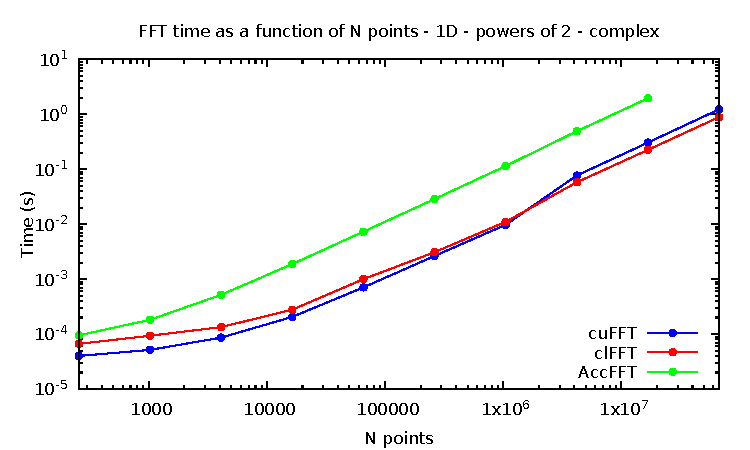
\includegraphics[width=.9\linewidth]{graphs/fft-1d-pow2-c-exec.pdf}
\caption{Execution (complex)}
\label{FFTPOW21DCE}
\end{subfigure}
\caption{Initialisation and execution times as a function of the number of points (1 dimension, powers of 2)}
\label{FFTPOW21D}
\end{figure}


\begin{figure}[H]
\captionsetup{width=0.8\linewidth}
\centering
\begin{subfigure}{.5\textwidth}
\centering
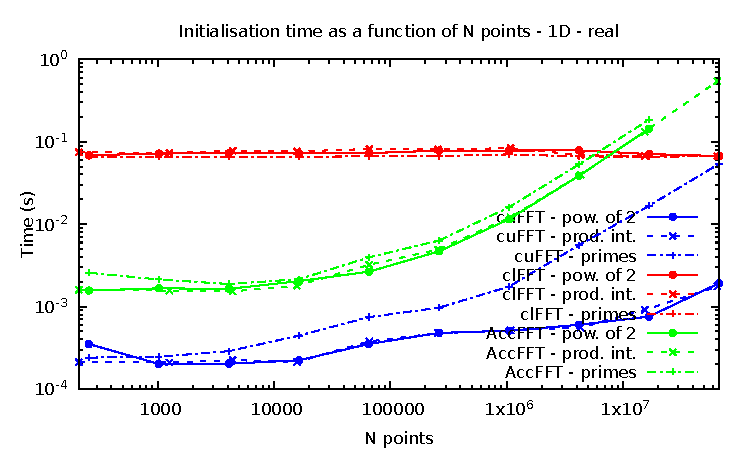
\includegraphics[width=.9\linewidth]{graphs/fft-1d-r-init.pdf}
\caption{Intialisation (real)}
\label{FFT1DRI}
\end{subfigure}%
\begin{subfigure}{.5\textwidth}
\centering
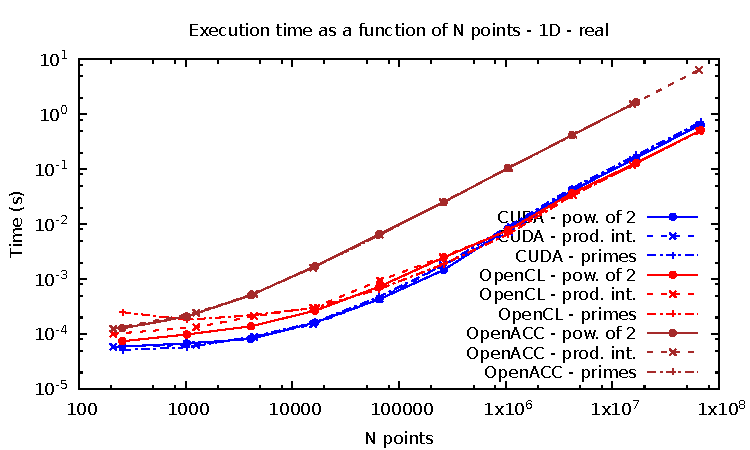
\includegraphics[width=.9\linewidth]{graphs/fft-1d-r-exec.pdf}
\caption{Execution (real)}
\label{FFT1DRE}
\end{subfigure}\\
\begin{subfigure}{.5\textwidth}
\centering
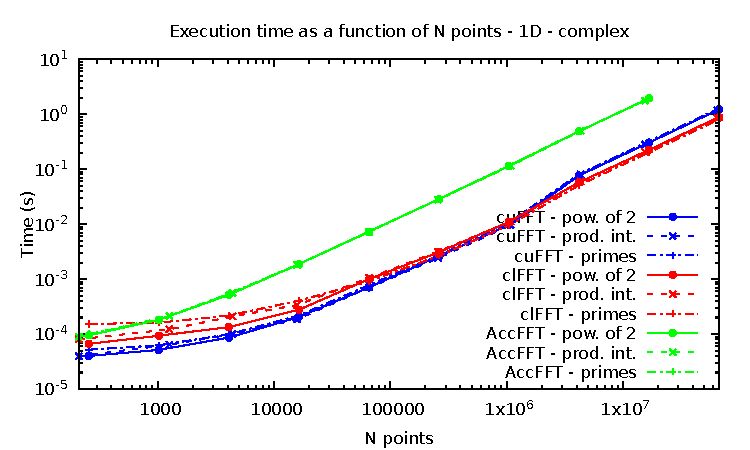
\includegraphics[width=.9\linewidth]{graphs/fft-1d-c-exec.pdf}
\caption{Intialisation (complex)}
\label{FFT1DCI}
\end{subfigure}%
\begin{subfigure}{.5\textwidth}
\centering
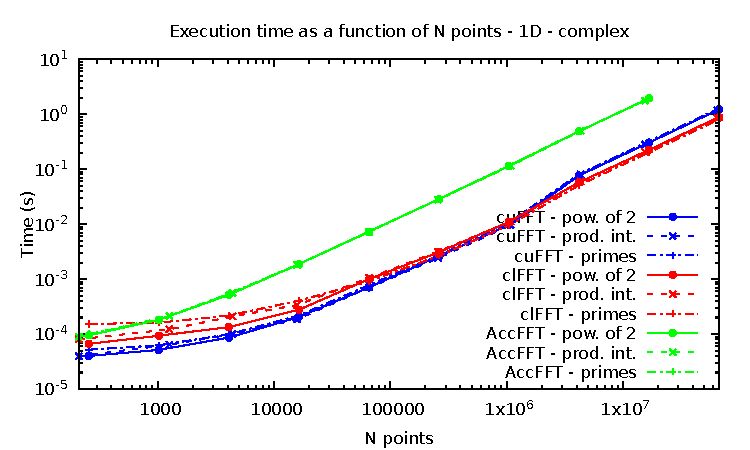
\includegraphics[width=.9\linewidth]{graphs/fft-1d-c-exec.pdf}
\caption{Execution (complex)}
\label{FFT1DCE}
\end{subfigure}
\caption{Initialisation and execution times as a function of the number of points (1 dimension)}
\label{FFT1D}
\end{figure}

\begin{figure}[H]
\captionsetup{width=0.8\linewidth}
\centering
\begin{subfigure}{.5\textwidth}
\centering
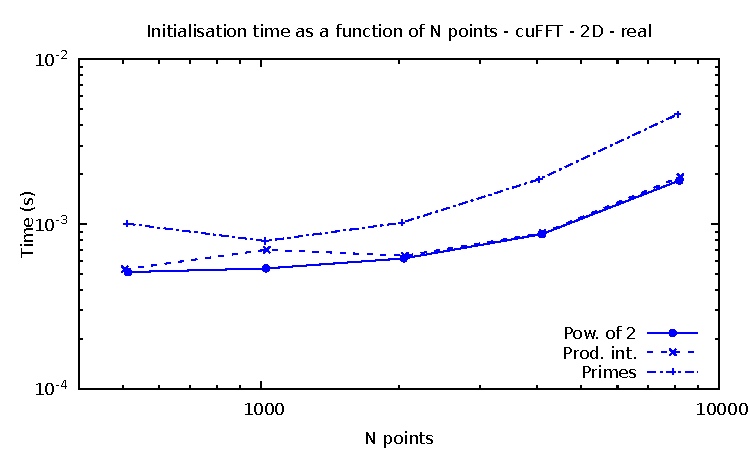
\includegraphics[width=.9\linewidth]{graphs/fft-cuda-2d-pow2-r-init.pdf}
\caption{Intialisation (real)}
\label{FFTCUDA2DRI}
\end{subfigure}%
\begin{subfigure}{.5\textwidth}
\centering
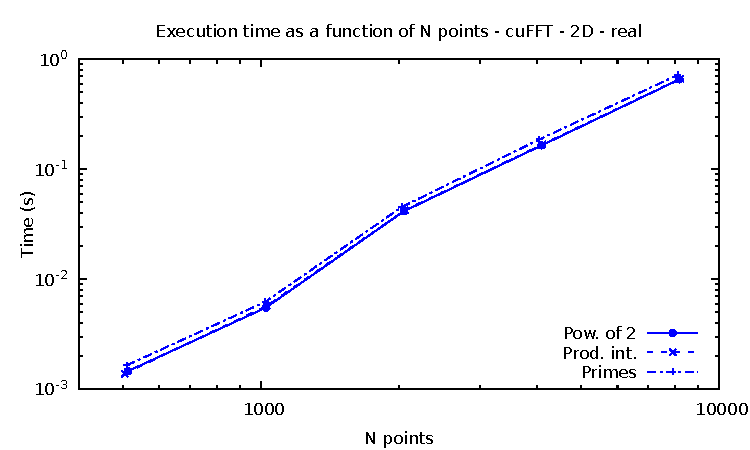
\includegraphics[width=.9\linewidth]{graphs/fft-cuda-2d-pow2-r-exec.pdf}
\caption{Execution (real)}
\label{FFTCUDA2DRE}
\end{subfigure}\\
\begin{subfigure}{.5\textwidth}
\centering
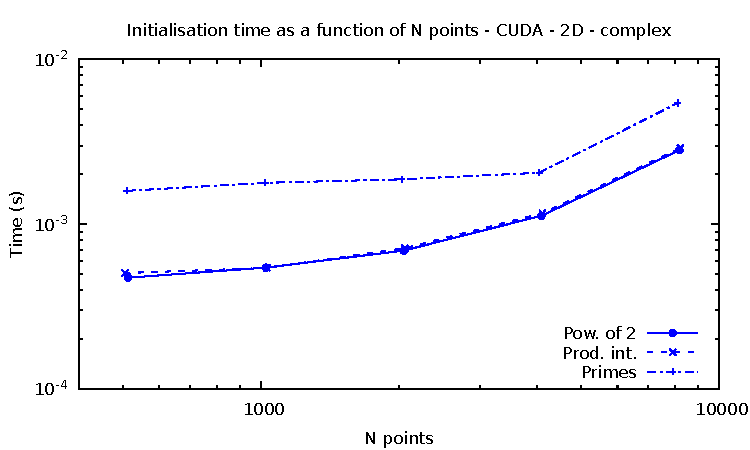
\includegraphics[width=.9\linewidth]{graphs/fft-cuda-2d-pow2-c-init.pdf}
\caption{Intialisation (complex)}
\label{FFTCUDA2DCI}
\end{subfigure}%
\begin{subfigure}{.5\textwidth}
\centering
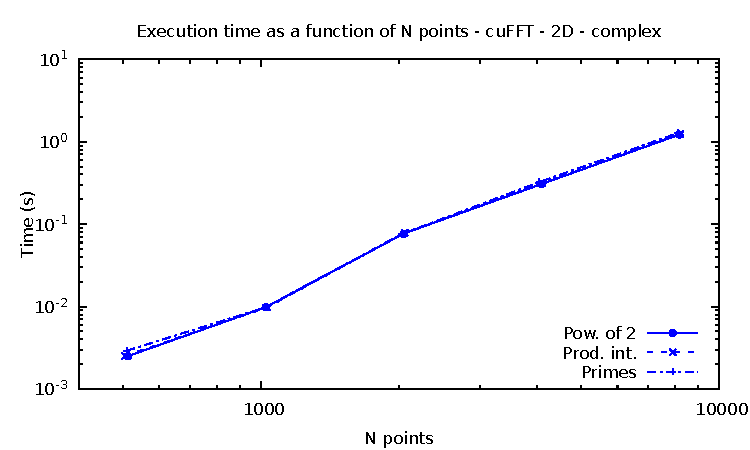
\includegraphics[width=.9\linewidth]{graphs/fft-cuda-2d-pow2-c-exec.pdf}
\caption{Execution (complex)}
\label{FFTCUDA2DCE}
\end{subfigure}
\caption{Initialisation and execution times as a function of the number of points\\(CUDA, 2 dimension)}
\label{FFTCUDA2D}
\end{figure}

\begin{figure}[H]
\captionsetup{width=0.8\linewidth}
\centering
\begin{subfigure}{.5\textwidth}
\centering
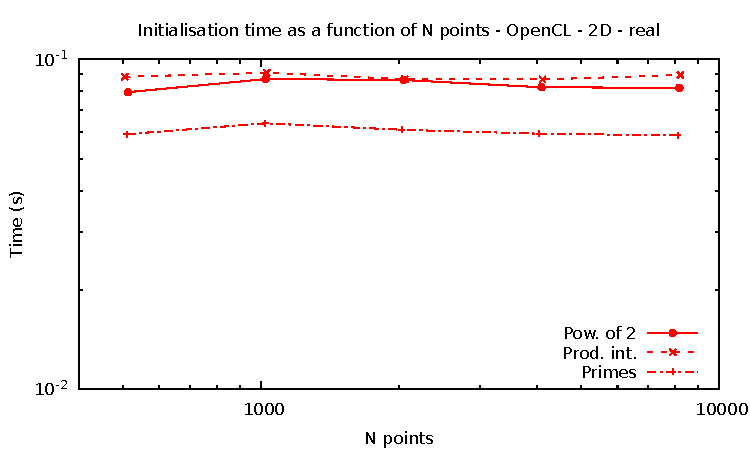
\includegraphics[width=.9\linewidth]{graphs/fft-opencl-2d-pow2-r-init.pdf}
\caption{Intialisation (real)}
\label{FFTCL2DRI}
\end{subfigure}%
\begin{subfigure}{.5\textwidth}
\centering
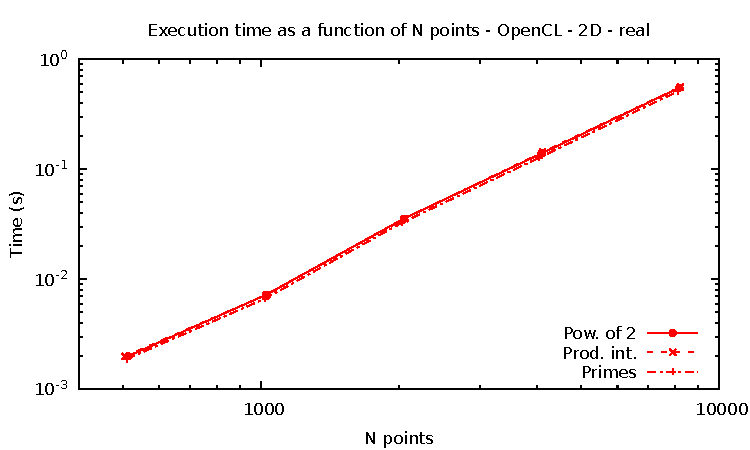
\includegraphics[width=.9\linewidth]{graphs/fft-opencl-2d-pow2-r-exec.pdf}
\caption{Execution (real)}
\label{FFTCL2DRE}
\end{subfigure}\\
\begin{subfigure}{.5\textwidth}
\centering
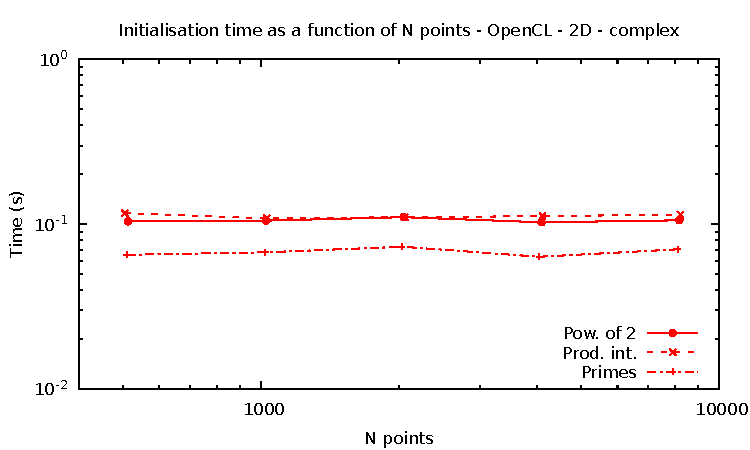
\includegraphics[width=.9\linewidth]{graphs/fft-opencl-2d-pow2-c-init.pdf}
\caption{Intialisation (complex)}
\label{FFTCL2DCI}
\end{subfigure}%
\begin{subfigure}{.5\textwidth}
\centering
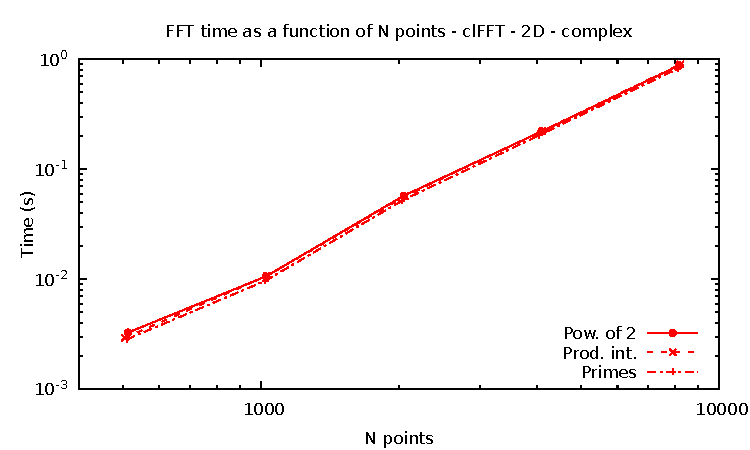
\includegraphics[width=.9\linewidth]{graphs/fft-opencl-2d-pow2-c-exec.pdf}
\caption{Execution (complex)}
\label{FFTCL2DCE}
\end{subfigure}
\caption{Initialisation and execution times as a function of the number of points\\(OpenCL, 1 dimension)}
\label{FFTCL2D}
\end{figure}


\begin{figure}[H]
\captionsetup{width=0.8\linewidth}
\centering
\begin{subfigure}{.5\textwidth}
\centering
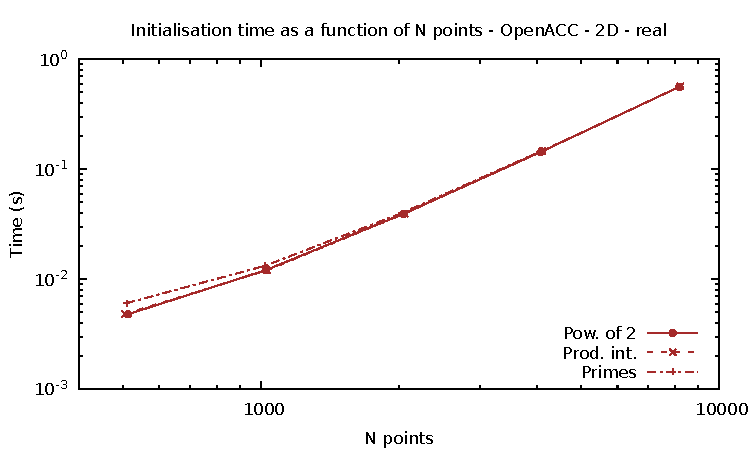
\includegraphics[width=.9\linewidth]{graphs/fft-openacc-2d-pow2-r-init.pdf}
\caption{Intialisation (real)}
\label{FFTACC2DRI}
\end{subfigure}%
\begin{subfigure}{.5\textwidth}
\centering
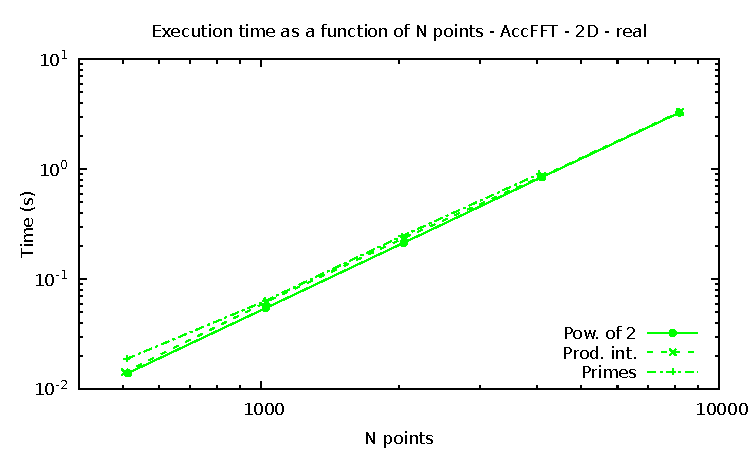
\includegraphics[width=.9\linewidth]{graphs/fft-openacc-2d-pow2-r-exec.pdf}
\caption{Execution (real)}
\label{FFTACC2DRE}
\end{subfigure}\\
\begin{subfigure}{.5\textwidth}
\centering
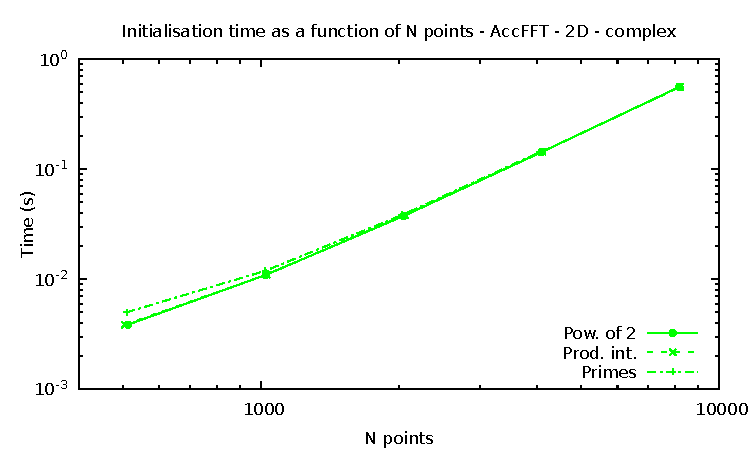
\includegraphics[width=.9\linewidth]{graphs/fft-openacc-2d-pow2-c-init.pdf}
\caption{Intialisation (complex)}
\label{FFTACC2DCI}
\end{subfigure}%
\begin{subfigure}{.5\textwidth}
\centering
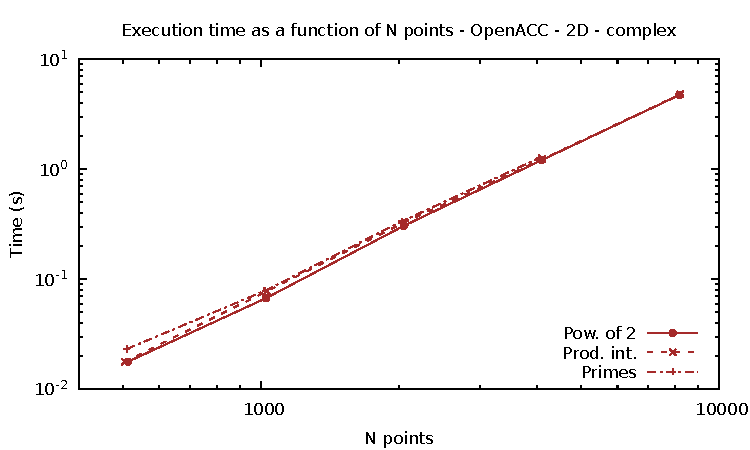
\includegraphics[width=.9\linewidth]{graphs/fft-openacc-2d-pow2-c-exec.pdf}
\caption{Execution (complex)}
\label{FFTACC2DCE}
\end{subfigure}
\caption{Initialisation and execution times as a function of the number of points\\(OpenACC, 1 dimension)}
\label{FFTCL2D}
\end{figure}

\begin{figure}[H]
\captionsetup{width=0.8\linewidth}
\centering
\begin{subfigure}{.5\textwidth}
\centering
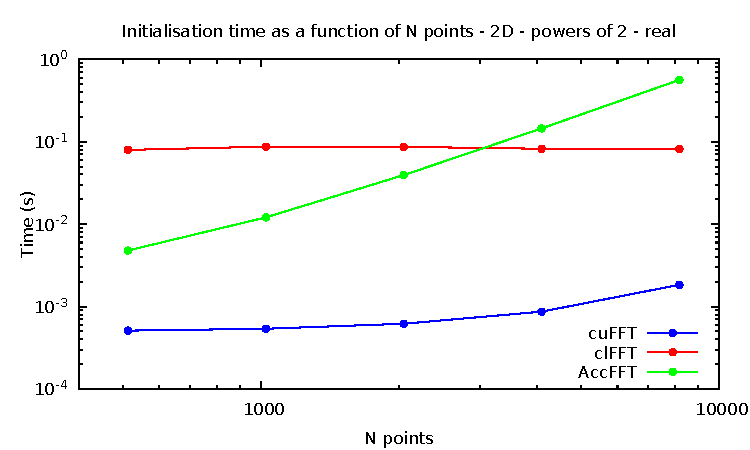
\includegraphics[width=.9\linewidth]{graphs/fft-2d-pow2-r-init.pdf}
\caption{Intialisation (real)}
\label{FFTPOW22DRI}
\end{subfigure}%
\begin{subfigure}{.5\textwidth}
\centering
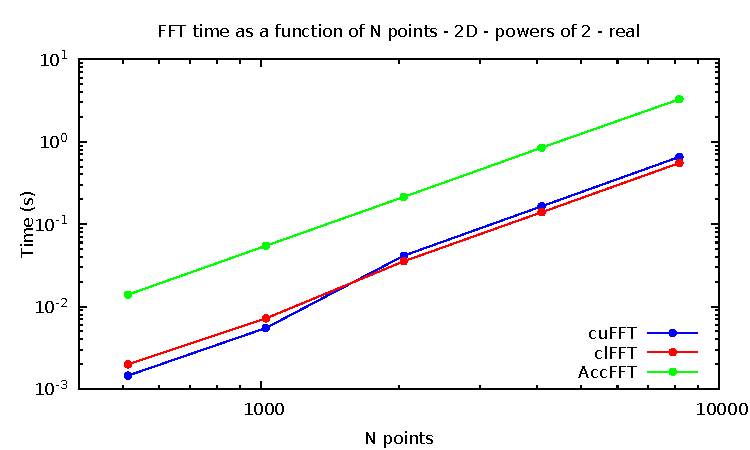
\includegraphics[width=.9\linewidth]{graphs/fft-2d-pow2-r-exec.pdf}
\caption{Execution (real)}
\label{FFTPOW22DRE}
\end{subfigure}\\
\begin{subfigure}{.5\textwidth}
\centering
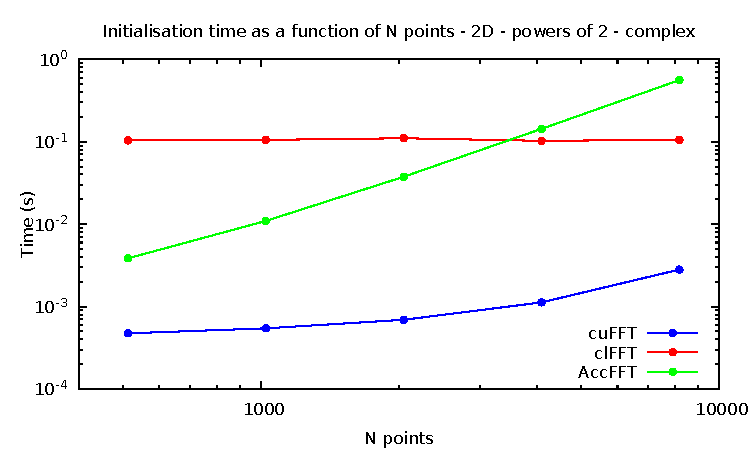
\includegraphics[width=.9\linewidth]{graphs/fft-2d-pow2-c-init.pdf}
\caption{Intialisation (complex)}
\label{FFTPOW22DCI}
\end{subfigure}%
\begin{subfigure}{.5\textwidth}
\centering
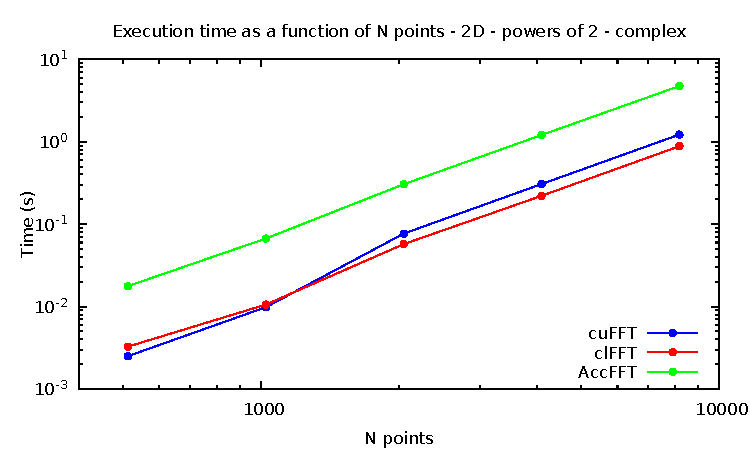
\includegraphics[width=.9\linewidth]{graphs/fft-2d-pow2-c-exec.pdf}
\caption{Execution (complex)}
\label{FFTPOW22DCE}
\end{subfigure}
\caption{Initialisation and execution times as a function of the number of points\\(1 dimension, powers of 2)}
\label{FFTPOW22D}
\end{figure}

\begin{figure}[H]
\captionsetup{width=0.8\linewidth}
\centering
\begin{subfigure}{.5\textwidth}
\centering
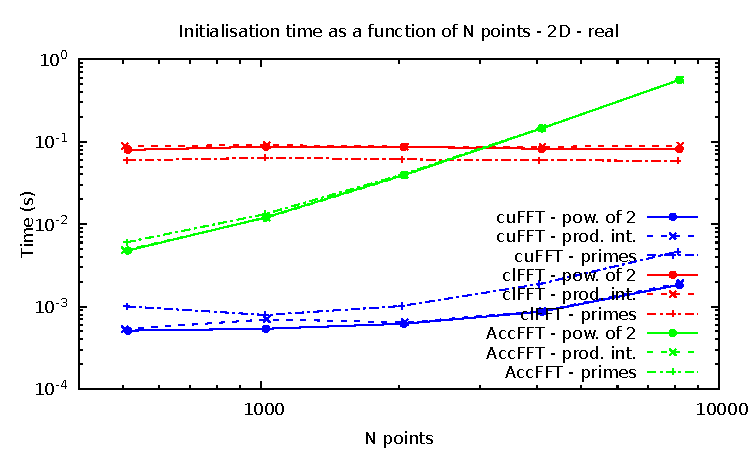
\includegraphics[width=.9\linewidth]{graphs/fft-2d-r-init.pdf}
\caption{Intialisation (real)}
\label{FFT2DRI}
\end{subfigure}%
\begin{subfigure}{.5\textwidth}
\centering
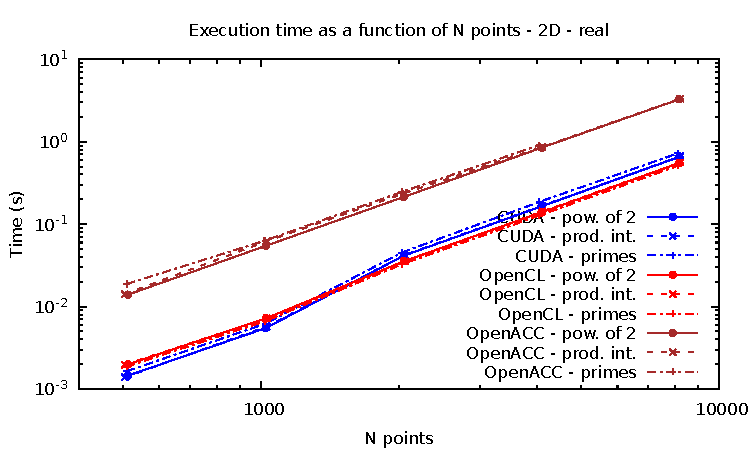
\includegraphics[width=.9\linewidth]{graphs/fft-2d-r-exec.pdf}
\caption{Execution (real)}
\label{FFT2DRE}
\end{subfigure}\\
\begin{subfigure}{.5\textwidth}
\centering
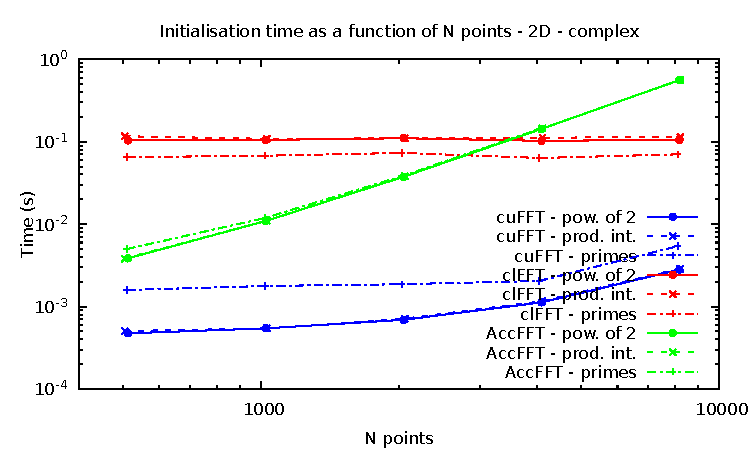
\includegraphics[width=.9\linewidth]{graphs/fft-2d-c-init.pdf}
\caption{Intialisation (complex)}
\label{FFT2DCI}
\end{subfigure}%
\begin{subfigure}{.5\textwidth}
\centering
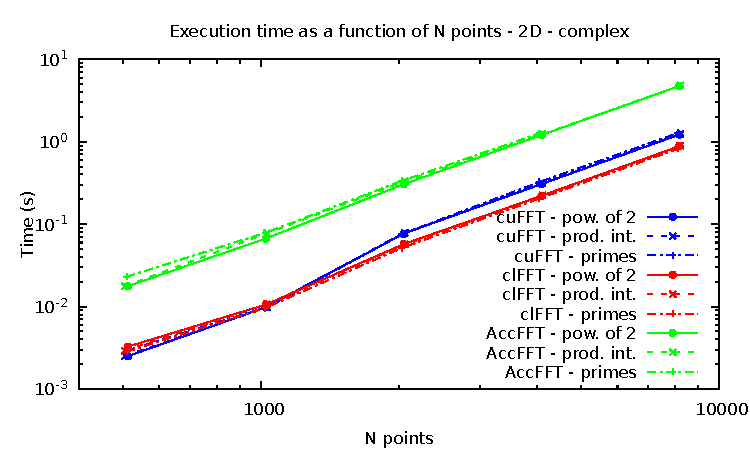
\includegraphics[width=.9\linewidth]{graphs/fft-2d-c-exec.pdf}
\caption{Execution (complex)}
\label{FFT2DCE}
\end{subfigure}
\caption{Initialisation and execution times as a function of the number of points\\(2 dimensions)}
\label{FFT1D}
\end{figure}

\begin{figure}[H]
\captionsetup{width=0.8\linewidth}
\centering
\begin{subfigure}{.5\textwidth}
\centering
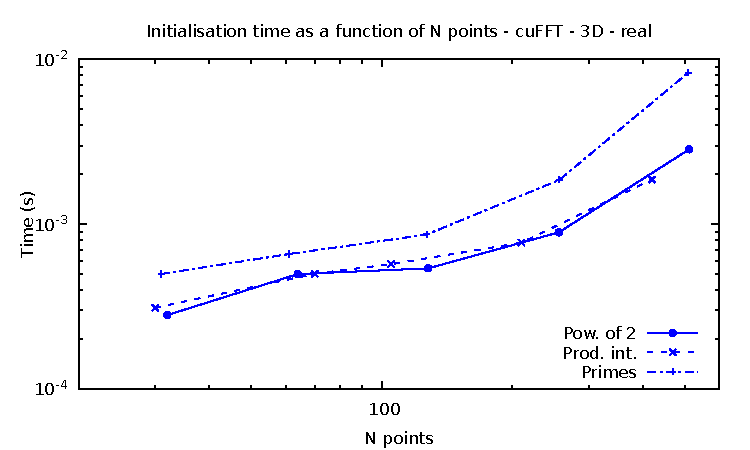
\includegraphics[width=.9\linewidth]{graphs/fft-cuda-3d-pow2-r-init.pdf}
\caption{Intialisation (real)}
\label{FFTCUDA3DRI}
\end{subfigure}%
\begin{subfigure}{.5\textwidth}
\centering
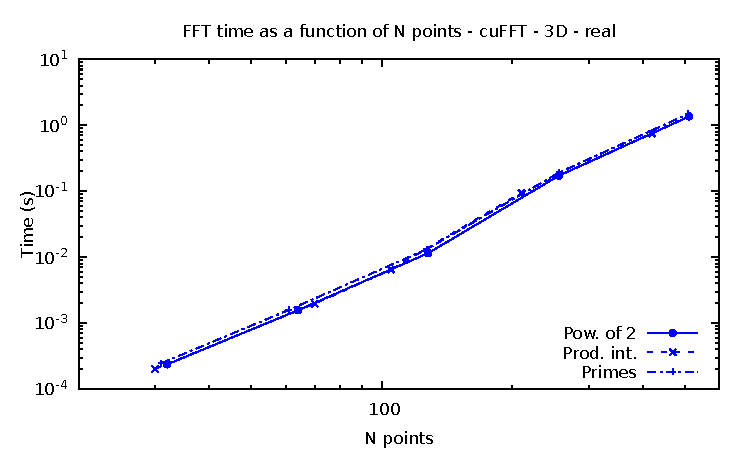
\includegraphics[width=.9\linewidth]{graphs/fft-cuda-3d-pow2-r-exec.pdf}
\caption{Execution (real)}
\label{FFTCUDA3DRE}
\end{subfigure}\\
\begin{subfigure}{.5\textwidth}
\centering
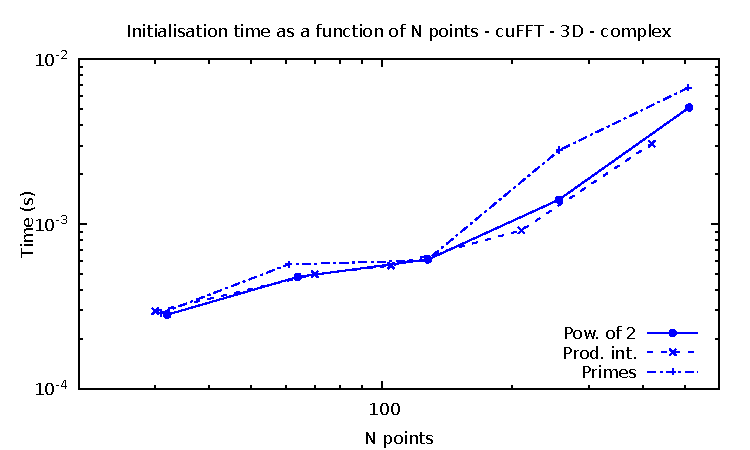
\includegraphics[width=.9\linewidth]{graphs/fft-cuda-3d-pow2-c-init.pdf}
\caption{Intialisation (complex)}
\label{FFTCUDA3DCI}
\end{subfigure}%
\begin{subfigure}{.5\textwidth}
\centering
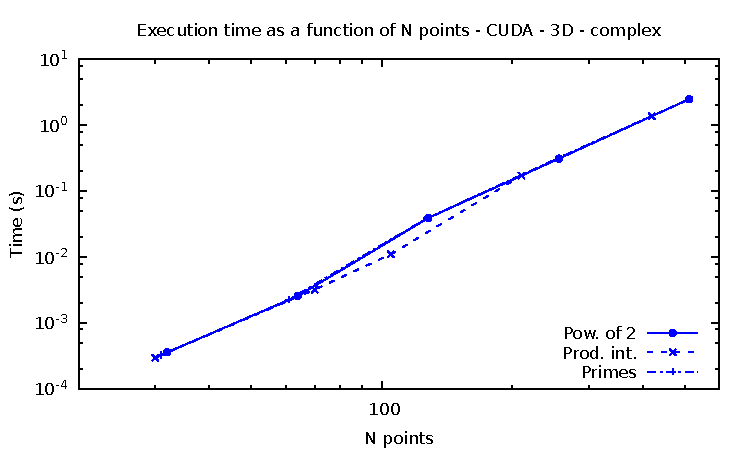
\includegraphics[width=.9\linewidth]{graphs/fft-cuda-3d-pow2-c-exec.pdf}
\caption{Execution (complex)}
\label{FFTCUDA3DCE}
\end{subfigure}
\caption{Initialisation and execution times as a function of the number of points (CUDA, 3 dimensions)}
\label{FFTCUDA3D}
\end{figure}

\begin{figure}[H]
\captionsetup{width=0.8\linewidth}
\centering
\begin{subfigure}{.5\textwidth}
\centering
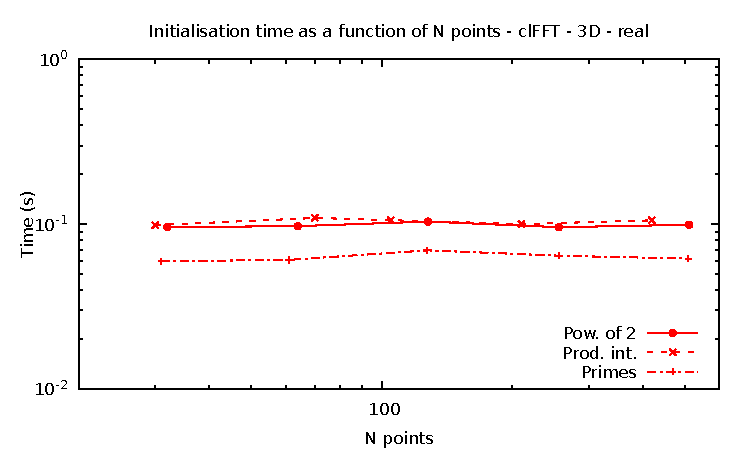
\includegraphics[width=.9\linewidth]{graphs/fft-opencl-3d-pow2-r-init.pdf}
\caption{Intialisation (real)}
\label{FFTCL3DRI}
\end{subfigure}%
\begin{subfigure}{.5\textwidth}
\centering
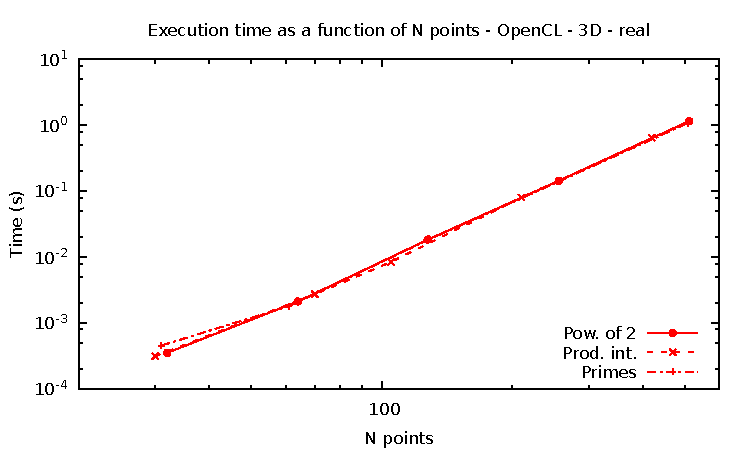
\includegraphics[width=.9\linewidth]{graphs/fft-opencl-3d-pow2-r-exec.pdf}
\caption{Execution (real)}
\label{FFTCL3DRE}
\end{subfigure}\\
\begin{subfigure}{.5\textwidth}
\centering
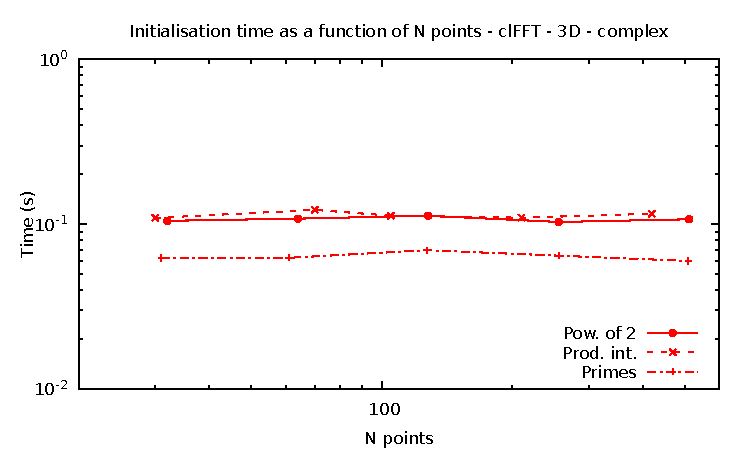
\includegraphics[width=.9\linewidth]{graphs/fft-opencl-3d-pow2-c-init.pdf}
\caption{Intialisation (complex)}
\label{FFTCL3DCI}
\end{subfigure}%
\begin{subfigure}{.5\textwidth}
\centering
\includegraphics[width=.9\linewidth]{graphs/fft-opencl-3d-pow2-c-exec.pdf}
\caption{Execution (complex)}
\label{FFTCL3DCE}
\end{subfigure}
\caption{Initialisation and execution times as a function of the number of points (OpenCL, 1 dimension)}
\label{FFTCL3D}
\end{figure}

\begin{figure}[H]
\captionsetup{width=0.8\linewidth}
\centering
\begin{subfigure}{.5\textwidth}
\centering
\includegraphics[width=.9\linewidth]{graphs/fft-openacc-3d-pow2-r-init.pdf}
\caption{Intialisation (real)}
\label{FFTACC3DRI}
\end{subfigure}%
\begin{subfigure}{.5\textwidth}
\centering
\includegraphics[width=.9\linewidth]{graphs/fft-openacc-3d-pow2-r-exec.pdf}
\caption{Execution (real)}
\label{FFTACC3DRE}
\end{subfigure}\\
\begin{subfigure}{.5\textwidth}
\centering
\includegraphics[width=.9\linewidth]{graphs/fft-openacc-3d-pow2-c-init.pdf}
\caption{Intialisation (complex)}
\label{FFTACC3DCI}
\end{subfigure}%
\begin{subfigure}{.5\textwidth}
\centering
\includegraphics[width=.9\linewidth]{graphs/fft-openacc-3d-pow2-c-exec.pdf}
\caption{Execution (complex)}
\label{FFTACC3DCE}
\end{subfigure}
\caption{Initialisation and execution times as a function of the number of points (OpenACC, 3 dimension)}
\label{FFTCL3D}
\end{figure}

\begin{figure}[H]
\captionsetup{width=0.8\linewidth}
\centering
\begin{subfigure}{.5\textwidth}
\centering
\includegraphics[width=.9\linewidth]{graphs/fft-3d-pow2-r-init.pdf}
\caption{Intialisation (real)}
\label{FFTPOW23DRI}
\end{subfigure}%
\begin{subfigure}{.5\textwidth}
\centering
\includegraphics[width=.9\linewidth]{graphs/fft-3d-pow2-r-exec.pdf}
\caption{Execution (real)}
\label{FFTPOW23DRE}
\end{subfigure}\\
\begin{subfigure}{.5\textwidth}
\centering
\includegraphics[width=.9\linewidth]{graphs/fft-3d-pow2-c-init.pdf}
\caption{Intialisation (complex)}
\label{FFTPOW23DCI}
\end{subfigure}%
\begin{subfigure}{.5\textwidth}
\centering
\includegraphics[width=.9\linewidth]{graphs/fft-3d-pow2-c-exec.pdf}
\caption{Execution (complex)}
\label{FFTPOW23DCE}
\end{subfigure}
\caption{Initialisation and execution times as a function of the number of points (3 dimensions, powers of 2)}
\label{FFTPOW23D}
\end{figure}

\begin{figure}[H]
\captionsetup{width=0.8\linewidth}
\centering
\begin{subfigure}{.5\textwidth}
\centering
\includegraphics[width=.9\linewidth]{graphs/fft-3d-r-init.pdf}
\caption{Intialisation (real)}
\label{FFT3DRI}
\end{subfigure}%
\begin{subfigure}{.5\textwidth}
\centering
\includegraphics[width=.9\linewidth]{graphs/fft-3d-r-exec.pdf}
\caption{Execution (real)}
\label{FFT3DRE}
\end{subfigure}\\
\begin{subfigure}{.5\textwidth}
\centering
\includegraphics[width=.9\linewidth]{graphs/fft-3d-c-init.pdf}
\caption{Intialisation (complex)}
\label{FFT3DCI}
\end{subfigure}%
\begin{subfigure}{.5\textwidth}
\centering
\includegraphics[width=.9\linewidth]{graphs/fft-3d-c-exec.pdf}
\caption{Execution (complex)}
\label{FFT3DCE}
\end{subfigure}
\caption{Initialisation and execution times as a function of the number of points (3 dimensions)}
\label{FFT3D}
\end{figure}

\subsection{Flatness}
So far, we have considered only square or cubic domains. In this section, we study the effect of the flatness of the domain by computing the FFT on a cuboid containing $256^3$. We define the flatmess by the ratio bewtween the number of points in the $y$ and $x$ directions whereas the dimensions in the $y$ and $z$ directions are identical (Flatness:=$N_y/N_x$, $N_y=N_z$). We observe that the flatness does not alter significantly the performance which remains dependent only on the total number of points.
\begin{figure}[H]
\captionsetup{width=0.8\linewidth}
\centering
\begin{subfigure}{.5\textwidth}
\centering
\includegraphics[width=.9\linewidth]{graphs/flatness-r-init.pdf}
\caption{Intialisation (real)}
\label{FFT1DRI}
\end{subfigure}%
\begin{subfigure}{.5\textwidth}
\centering
\includegraphics[width=.9\linewidth]{graphs/flatness-r-exec.pdf}
\caption{Execution (real)}
\label{FFT1DRE}
\end{subfigure}\\
\begin{subfigure}{.5\textwidth}
\centering
\includegraphics[width=.9\linewidth]{graphs/flatness-c-init.pdf}
\caption{Intialisation (complex)}
\label{FFT1DCI}
\end{subfigure}%
\begin{subfigure}{.5\textwidth}
\centering
\includegraphics[width=.9\linewidth]{graphs/flatness-c-exec.pdf}
\caption{Execution (complex)}
\label{FFT1DCE}
\end{subfigure}
\caption{Initialisation and execution times as a function of the number of points\\(1 dimension)}
\label{FFT1D}
\end{figure}
\subsection{CCPPETMR}
We have also benchmarked the libraries provided by these framework for the computation of FFTs in a context similar to the situation encountered by the CCP/PET-MR collaboration. In this example, we compute the FFT of 32 square complex images. Their side is made of 252, 256 and 256 points in the cases respectively of a number of points corresponding to the product of small integers, a power of 2 or a prime number. In this context, it is CUDA that is the most efficient.
\begin{figure}[H]
\captionsetup{width=0.8\linewidth}
\centering
\begin{subfigure}{.5\textwidth}
\centering
\includegraphics[width=.9\linewidth]{graphs/fft-ccppetmr-init.pdf}
\caption{Intialisation (real)}
\label{FFT1DRI}
\end{subfigure}%
\begin{subfigure}{.5\textwidth}
\centering
\includegraphics[width=.9\linewidth]{graphs/fft-ccppetmr-exec.pdf}
\caption{Execution (real)}
\label{FFT1DRE}
\end{subfigure}
\caption{Initialisation and execution times as a function of the number of points\\(1 dimension)}
\label{FFT1D}
\end{figure}s context, it is CUDA that is the most efficient. 




\section{Acknowledgements}

\begin{thebibliography}{9}

\bibitem{cuda}
\hyperlink{https://developer.nvidia.com/cuda-zone}{https://developer.nvidia.com/cuda-zone}

\bibitem{opencl}
\hyperlink{https://www.khronos.org/opencl/}{https://www.khronos.org/opencl/}
  
\bibitem{fftpack}
\hyperlink{https://www.khronos.org/opencl/}{https://www.khronos.org/opencl/}

\bibitem{openacc}
\hyperlink{https://www.openmp.org/}{https://www.openmp.org/}
  
\bibitem{openmp}
\hyperlink{https://www.openmp.org/}{https://www.openmp.org/}

\bibitem{kokkos}
\hyperlink{https://github.com/kokkos}{https://github.com/kokkos}

\bibitem{cufft}
\hyperlink{https://docs.nvidia.com/cuda/cufft/index.html}{https://docs.nvidia.com/cuda/cufft/index.html}

\bibitem{clfft}
  \hyperlink{https://github.com/clMathLibraries/clFFT}{https://github.com/clMathLibraries/clFFT}
  
\bibitem{accfft}
\hyperlink{http://accfft.org/}{http://accfft.org/}

\bibitem{casa}
McMullin, J. P., Waters, B., Schiebel, D., Young, W., Golap, K.,
{\it Astronomical Data Analysis Software and Systems XVI},
ASP Conf. Ser. 376, ed. R. A. Shaw, F. Hill, D. J. Bell (San Francisco, CA: ASP), 127

\bibitem{code}
\hyperlink{git@github.com:SoftwareOutlook/GPU.git}{git@github.com:SoftwareOutlook/GPU.git}
    
\bibitem{ccppetmr}
\hyperlink{https://www.ccppetmr.ac.uk/}{https://www.ccppetmr.ac.uk/}

\bibitem{softwareoutlook}
\hyperlink{https://www.softwareoutlook.ac.uk/}{https://www.softwareoutlook.ac.uk/}
  
\end{thebibliography}

\end{document}
